\begin{center}
\section{Enfoque del problema}
\end{center}

\justify
\noindent
Existen en el mercado actual productos de origen biol\'ogico cuya obtenci\'on parte de un mismo proceso productivo para sectores industriales como lo son el sector salud, agropecuario y cosm\'etico. Estos bioproductos presentan una gran demanda en el mercado, tanto nacional como internacional, debido a que cuentan con diferentes propiedades qu\'imicas que los hacen competitivos frente a su contraparte sint\'etica.

\noindent
\justify

Se han realizado m\'ultiples estudios cient\'ificos a las propiedades biol\'ologicas de la flora colombiana referente a las hojas, tallos, ra\'ices, semillas y flores de distintas especies vegetales; destac\'andose los metabolitos y flavonoides, encontradas en hojas y flores, que presentan actividad antimicrobiana, antibacterial, antif\'ungica, antioxidante e insecticida, por mencionar algunas.

\noindent
\justify

Por estas razones, Colciencias, a trav\'es de la convocatoria de Colombia Cient\'ifica, aval\'o el programa 'Bio-Reto XXI - 15:50', que se trata de un proyecto que busca impulsar la producci\'on a mediana y gran escala de ingredientes naturales, tanto a nivel nacional como internacional, para mejorar la competitividad de diferentes industrias y directamente la econom\'ia del pa\'is. B\'asicamente, se trata del dise\~no y construcci\'on de una biof\'abrica destinada a la producci\'on de \textit{aceite esencial} y \textit{extracto} de origen vegetal, como se aprecia en la Figura \ref{cadena}. 

\noindent
\justify

\begin{figure}[h!]
	\centering
	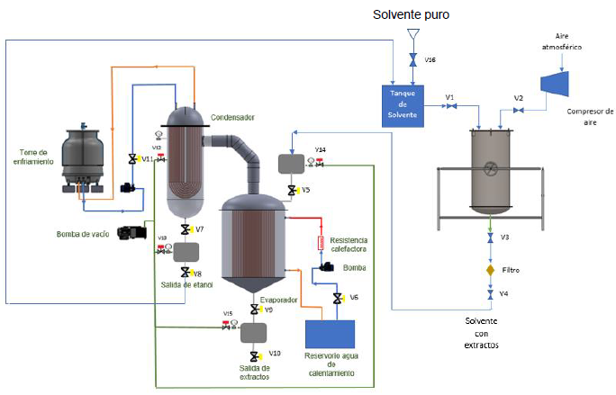
\includegraphics[width=0.85\textwidth]{Images/planta.PNG}
	\caption{Cadena productiva de la biof\'abrica.}
	\label{cadena}
\end{figure}

\newpage

\noindent
\justify

De la Figura \ref{cadena}:

\begin{itemize}
	\item $m_v \rightarrow $ Material vegetal.
	\item $m_p \rightarrow $ Material pulverizado (mezcla entre el material vegetal con el agente dispersante).
	\item $FS \rightarrow $ Fase s\'olida. Corresponde al residuo del material pulverizado despu\'es de la extracci\'on.
	\item $FL \rightarrow $ Fase l\'iquida. Corresponde a la mezcla l\'iquida homog\'enea entre el solvente y el extracto.
\end{itemize}

\noindent
\justify

El \textit{objeto} de estudio del presente trabajo se centra en el sistema de eluci\'on y filtrado de la planta de extracci\'on, que tiene por \textit{objetivo} separar el extracto del material vegetal pulverizado.

